% Options for packages loaded elsewhere
\PassOptionsToPackage{unicode}{hyperref}
\PassOptionsToPackage{hyphens}{url}
%
\documentclass[
]{report}
\usepackage{lmodern}
\usepackage{amssymb,amsmath}
\usepackage{ifxetex,ifluatex}
\ifnum 0\ifxetex 1\fi\ifluatex 1\fi=0 % if pdftex
  \usepackage[T1]{fontenc}
  \usepackage[utf8]{inputenc}
  \usepackage{textcomp} % provide euro and other symbols
\else % if luatex or xetex
  \usepackage{unicode-math}
  \defaultfontfeatures{Scale=MatchLowercase}
  \defaultfontfeatures[\rmfamily]{Ligatures=TeX,Scale=1}
\fi
% Use upquote if available, for straight quotes in verbatim environments
\IfFileExists{upquote.sty}{\usepackage{upquote}}{}
\IfFileExists{microtype.sty}{% use microtype if available
  \usepackage[]{microtype}
  \UseMicrotypeSet[protrusion]{basicmath} % disable protrusion for tt fonts
}{}
\makeatletter
\@ifundefined{KOMAClassName}{% if non-KOMA class
  \IfFileExists{parskip.sty}{%
    \usepackage{parskip}
  }{% else
    \setlength{\parindent}{0pt}
    \setlength{\parskip}{6pt plus 2pt minus 1pt}}
}{% if KOMA class
  \KOMAoptions{parskip=half}}
\makeatother
\usepackage{xcolor}
\IfFileExists{xurl.sty}{\usepackage{xurl}}{} % add URL line breaks if available
\IfFileExists{bookmark.sty}{\usepackage{bookmark}}{\usepackage{hyperref}}
\hypersetup{
  pdftitle={  STAT 216 Activity Coursepack},
  hidelinks,
  pdfcreator={LaTeX via pandoc}}
\urlstyle{same} % disable monospaced font for URLs
\usepackage{longtable,booktabs}
% Correct order of tables after \paragraph or \subparagraph
\usepackage{etoolbox}
\makeatletter
\patchcmd\longtable{\par}{\if@noskipsec\mbox{}\fi\par}{}{}
\makeatother
% Allow footnotes in longtable head/foot
\IfFileExists{footnotehyper.sty}{\usepackage{footnotehyper}}{\usepackage{footnote}}
\makesavenoteenv{longtable}
\usepackage{graphicx,grffile}
\makeatletter
\def\maxwidth{\ifdim\Gin@nat@width>\linewidth\linewidth\else\Gin@nat@width\fi}
\def\maxheight{\ifdim\Gin@nat@height>\textheight\textheight\else\Gin@nat@height\fi}
\makeatother
% Scale images if necessary, so that they will not overflow the page
% margins by default, and it is still possible to overwrite the defaults
% using explicit options in \includegraphics[width, height, ...]{}
\setkeys{Gin}{width=\maxwidth,height=\maxheight,keepaspectratio}
% Set default figure placement to htbp
\makeatletter
\def\fps@figure{htbp}
\makeatother
\setlength{\emergencystretch}{3em} % prevent overfull lines
\providecommand{\tightlist}{%
  \setlength{\itemsep}{0pt}\setlength{\parskip}{0pt}}
\setcounter{secnumdepth}{-\maxdimen} % remove section numbering
\usepackage{booktabs}
\usepackage{geometry}
\usepackage[none]{hyphenat}

\pagestyle{plain}

%%%% Set margins?... doesn't work
%\setlength{\topmargin}{-1cm}
%\addtolength{\evensidemargin}{-1cm}
%\addtolength{\oddsidemargin}{-1cm}
%\addtolength{\textheight}{1.8cm}
%\addtolength{\textwidth}{2cm}
\usepackage[]{natbib}
\bibliographystyle{plainnat}

\title{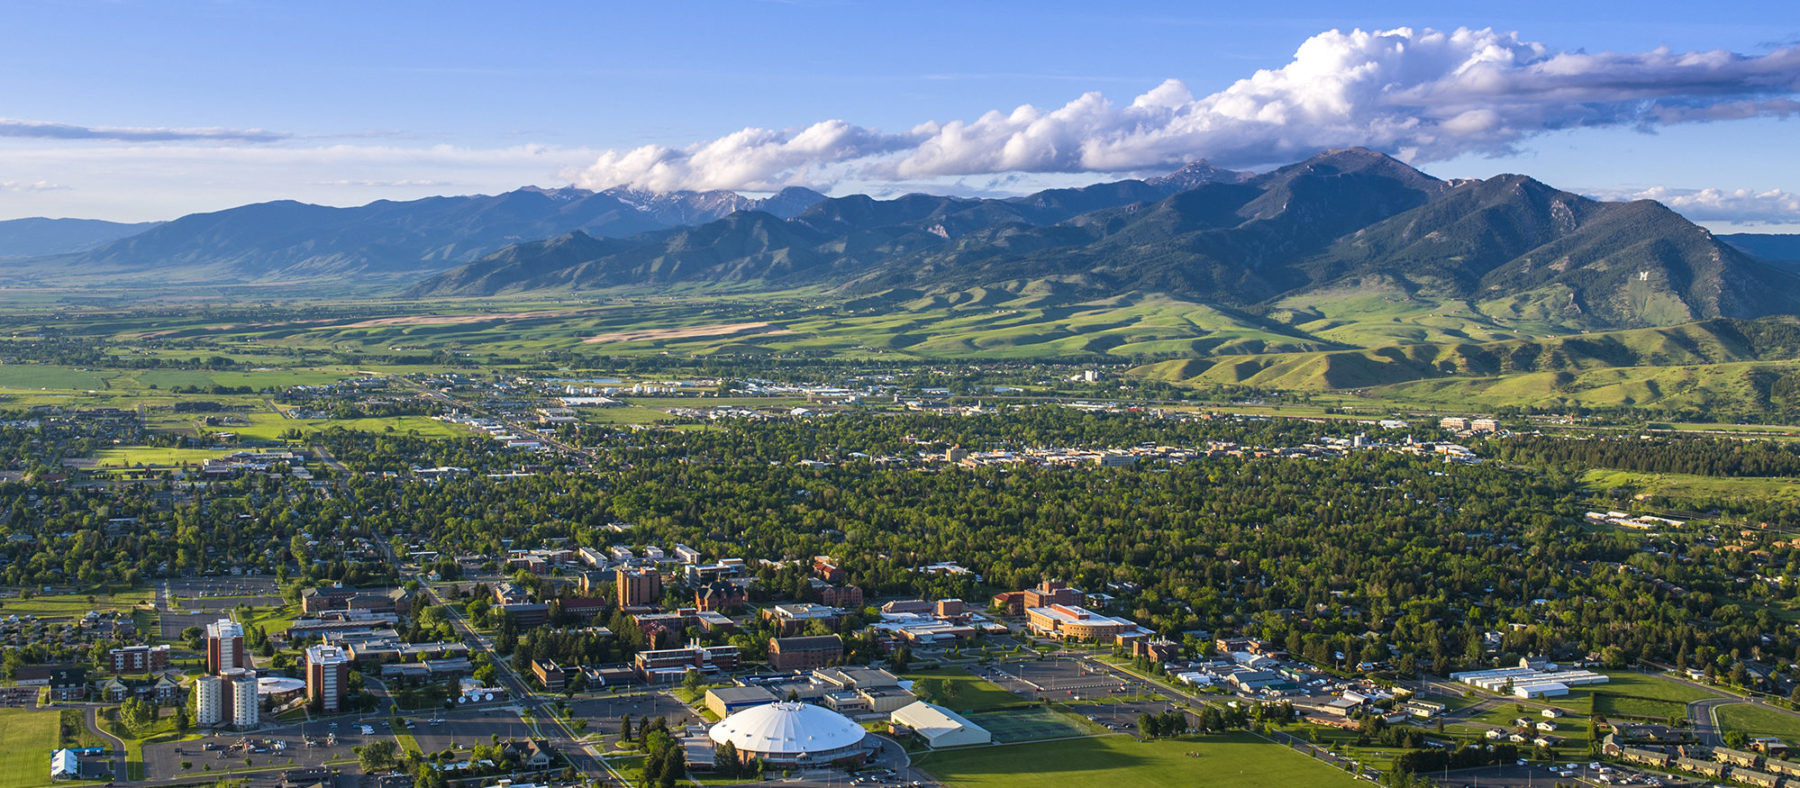
\includegraphics[width=5in,height=\textheight]{images/msu-campus.jpg}
\vspace{1cm}\\
STAT 216 Activity Coursepack}
\usepackage{etoolbox}
\makeatletter
\providecommand{\subtitle}[1]{% add subtitle to \maketitle
  \apptocmd{\@title}{\par {\large #1 \par}}{}{}
}
\makeatother
\subtitle{Fall 2020}
\author{}
\date{\vspace{-2.5em}}

\begin{document}
\maketitle

{
\setcounter{tocdepth}{0}
\tableofcontents
}
\hypertarget{preface}{%
\chapter{Preface}\label{preface}}

This coursepack accompanies the textbook for STAT 216: Introduction to Statistics at Montana State University. Each of the activities in this workbook is designed to target specific learning outcomes of the course, giving you practice with important statistical concepts in a group setting with instructor guidance. Bring this workbook with you to class each week, and take notes in the workbook as you would your own notes. A well-written complete workbook will provide an optimal study guide for exams!

\hypertarget{martian-alphabet}{%
\chapter{Martian Alphabet}\label{martian-alphabet}}

\hypertarget{learning-outcomes}{%
\section{Learning Outcomes}\label{learning-outcomes}}

\begin{itemize}
\item
  Describe the statistical investigation process
\item
  Identify observational units, variables, and variable types in a statistical study
\end{itemize}

How well can humans distinguish one ``Martian'' letter from another? In today's activity, we'll find out. When shown the two Martian letters, kiki and bumba, write down whether you think bumba is on the left or the right.

\vspace{0.5in}

\hypertarget{steps-of-statistical-investigation}{%
\section{Steps of Statistical Investigation}\label{steps-of-statistical-investigation}}

The first step of any statistical investigation is to ask a research question. In this study the research question is: can we as a class read Martian? (we will refine this later on!). To answer any research question, we must design a study and collect data. (This will normally be provided for you in class.) For our question, the study consists of each student being presented with two Martian letters and asking which was bumba. Your responses will become our observed data that we will explore. To answer the research question we will simulate what \emph{could} have happened in our class given random chance, repeat that many times to understand the expected variability between different ``randomly guessing'' classes, then comparing our class's observed data to the simulation. This gives us an estimate of how often (or the probability of) our class's result would occur if we were all merely guessing, allowing us to determine if we as a class can in fact read Martian.

Let's explore the data.
\textbf{Observational units} or \textbf{cases} are the subjects data is collected on. In a data set the rows will represent a single observational unit.

\begin{enumerate}
\def\labelenumi{\arabic{enumi}.}
\tightlist
\item
  What are the observational units in this study?
\end{enumerate}

\vspace{0.5in}

\begin{enumerate}
\def\labelenumi{\arabic{enumi}.}
\setcounter{enumi}{1}
\tightlist
\item
  How many students are in class today? This is the sample size.
\end{enumerate}

\vspace{0.5in}

A \textbf{variable} is information collected or measured on each observational unit or case. We will look at two types of variables: \textbf{quantitative} and \textbf{categorical}. Each column in a data set will represent a different variable.

Quantitative variables are numerical measurements that can be discrete (whole, non-negative numbers) or continuous (any value within an interval). The number of students in a class would be a discrete variable as you can not have a partial student. GPA would be a continuous variable ranging from 0 to 4.0.

Categorical variables are data that are in groups or categories such as eye color, state of residency, or whether or not a student is considered in-state. Categorical variables with a natural ordering are considered ordinal variables while those without a natural ordering are considered a nominal variable. All variables will be treated as nominal for analysis.

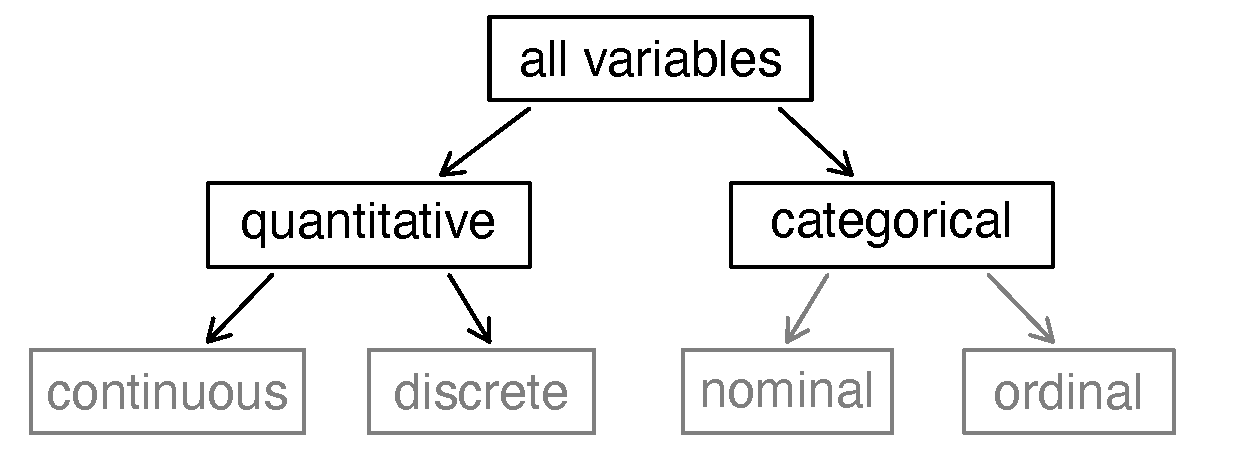
\includegraphics{images/variables.png}

\begin{enumerate}
\def\labelenumi{\arabic{enumi}.}
\setcounter{enumi}{2}
\tightlist
\item
  Identify the variable we are collecting on each observational unit in this study. What are we measuring on each student?
\end{enumerate}

\vspace{1in}

It is important to note that a variable is different than a summary statistic. A variable is measured on a \textbf{single observational unit} while a summary statistic is calculated from a group of observational units. For example, the variable \textbf{whether or not a student is considered in-state} can be measured on each individual student. In a class of 50 students we can calculate the proportion of students who are considered in-state, the summary statistic. Make sure you wrote the variable in question 3 as a variable \textbf{NOT} a summary statistic.

\begin{enumerate}
\def\labelenumi{\arabic{enumi}.}
\setcounter{enumi}{3}
\tightlist
\item
  Is the variable identified in question 3 categorical or quantitative?
\end{enumerate}

\vspace{0.5in}

\begin{enumerate}
\def\labelenumi{\arabic{enumi}.}
\setcounter{enumi}{4}
\tightlist
\item
  Were you correct or incorrect in identifying bumba?
\end{enumerate}

\vspace{0.5in}

We will now collect the data from the entire class.

\begin{enumerate}
\def\labelenumi{\arabic{enumi}.}
\setcounter{enumi}{5}
\tightlist
\item
  How many people in your class were correct in identifying bumba? Using the class size from question 2, calculate the proportion of students who correctly identified bumba.
\end{enumerate}

\begin{center}
$\mbox{proportion} = \frac{\mbox{number of students who correctly identified bumba}}{\mbox{total number of students}}$
\end{center}
\vspace{1in}

Looking at the data set and the summary statistics is only one way to display the data. We will also want to create a visualization or picture of the data. A \textbf{frequency bar plot} is used to display categorical data as a count or frequency. Since our variable has two levels, correct or incorrect, we will create two bars one for each level.

\begin{enumerate}
\def\labelenumi{\arabic{enumi}.}
\setcounter{enumi}{6}
\tightlist
\item
  Plot the observed class data using a frequency bar plot.
\end{enumerate}

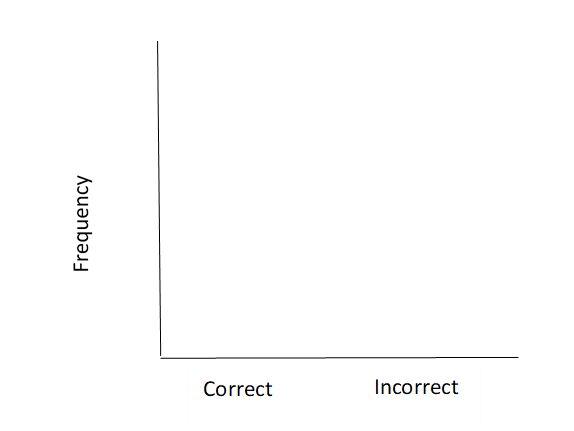
\includegraphics{images/barplot_martian.png}

We can also visualize the data as a proportion in a \textbf{relative frequency bar plot}. Relative frequency is the proportion calculated for each level of the categorical variable.

\begin{enumerate}
\def\labelenumi{\arabic{enumi}.}
\setcounter{enumi}{7}
\tightlist
\item
  Plot the observed class data using a relative frequency bar plot.
\end{enumerate}

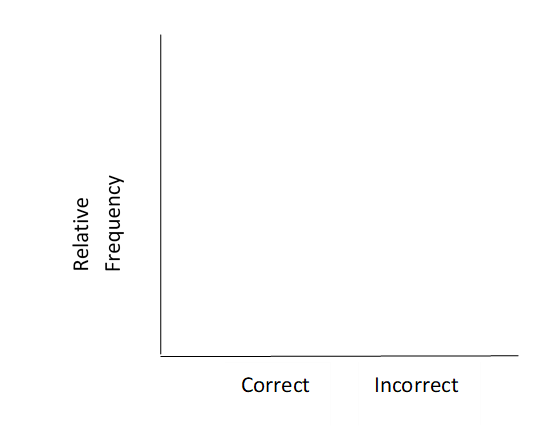
\includegraphics{images/relative_barplot_martian.png}

\newpage

\begin{enumerate}
\def\labelenumi{\arabic{enumi}.}
\setcounter{enumi}{8}
\tightlist
\item
  The next step is to analyze the data. If humans really don't know Martian and are just guessing which is bumba, what are the chances of getting it right?
  \vspace{0.5in}
\end{enumerate}

\begin{verbatim}
How could we use a coin to simulate each student “just guessing” which martian letter is bumba? 
\end{verbatim}

\vspace{1in}

\begin{verbatim}
How could we use coins to simulate the entire class “just guessing” which martian letter is bumba? 
\end{verbatim}

\vspace{1in}

\begin{verbatim}
How many people in your class would you expect to choose bumba correctly just by chance?  Explain your reasoning.
\end{verbatim}

\vspace{1in}

\begin{enumerate}
\def\labelenumi{\arabic{enumi}.}
\setcounter{enumi}{9}
\tightlist
\item
  Each of you will flip a coin one time to simulate your ``guess''. Let Heads = correct, Tails = incorrect. What was the result of your simulation? \vspace{1in}
\end{enumerate}

\begin{verbatim}
What was the result from your class’s simulation?  What proportion of students “guessed” correctly in the simulation?
\end{verbatim}

\vspace{1in}

\begin{enumerate}
\def\labelenumi{\arabic{enumi}.}
\setcounter{enumi}{10}
\tightlist
\item
  If students really don't know Martian and are just guessing which is bumba, which seems more unusual: the result from your class's \textbf{simulation} or the observed proportion of students in your class that were correct (this is your data from question 6)? Explain your reasoning.
\end{enumerate}

\vspace{1in}

\begin{enumerate}
\def\labelenumi{\arabic{enumi}.}
\setcounter{enumi}{11}
\tightlist
\item
  While your observed class data is likely far different from the simulated ``just-guessing'' class, comparing our class data to a single simulation does not seem to give enough information. The differences seen could just be due to that set of coin flips! Let's simulate another class. Each student should flip your coin again. What was the result from your class's second simulation? What proportion of students ``guessed'' correctly in the second simulation? Create a plot to compare the two simulated results with the observed class result.
\end{enumerate}

\vspace{1in}

\begin{enumerate}
\def\labelenumi{\arabic{enumi}.}
\setcounter{enumi}{12}
\tightlist
\item
  We still unfortunately only have a couple of simulations to compare our class data to. It would be much better to be able to see how our class compared to hundreds or thousands of ``just-guessing'' classes. Since we don't want to flip coins all class period, your instructor will use a computer simulation to get 1000 trials. Fill in the following blanks to describe how we would create a simulation of random guessing with 1000 trials.
  \vspace{0.1in}
\end{enumerate}

\begin{verbatim}
Probability of correct guesses: _____
\end{verbatim}

\vspace{0.1in}

\begin{verbatim}
Sample size: _____
\end{verbatim}

\vspace{0.1in}

\begin{verbatim}
Number of repetitions: _____
\end{verbatim}

\vspace{0.1in}

\begin{enumerate}
\def\labelenumi{\arabic{enumi}.}
\setcounter{enumi}{13}
\tightlist
\item
  Sketch the distribution displayed by your instructor here, being sure to label each axis appropriately.
\end{enumerate}

\vspace{2in}

\begin{enumerate}
\def\labelenumi{\arabic{enumi}.}
\setcounter{enumi}{14}
\tightlist
\item
  Is your class particularly good or bad at Martian? How can you use the plot in question 14 to tell?
\end{enumerate}

\vspace{1in}

\begin{enumerate}
\def\labelenumi{\arabic{enumi}.}
\setcounter{enumi}{15}
\tightlist
\item
  Is it possible that we could see our class results just by chance if everyone was just guessing? Explain your reasoning.
\end{enumerate}

\vspace{1in}

\begin{enumerate}
\def\labelenumi{\arabic{enumi}.}
\setcounter{enumi}{16}
\tightlist
\item
  Is it likely that we could see our class results just by chance if everyone was just guessing? Explain your reasoning.
\end{enumerate}

\vspace{1in}

\begin{enumerate}
\def\labelenumi{\arabic{enumi}.}
\setcounter{enumi}{17}
\tightlist
\item
  Does this activity provide strong evidence that students were not just guessing at random? If so, what do you think is going on here? Can we as a class read Martian?
\end{enumerate}

\vspace{1in}

\textbf{Take Home Messages}

\begin{enumerate}
\def\labelenumi{\arabic{enumi}.}
\item
  In this course we will learn how to evaluate a claim by comparing observed results (classes' ``guesses'') to a distribution of many simulated results under an assumption like ``blind guessing.''
\item
  Blind guessing between two outcomes will be correct only about half the time. We can create data (via computer simulation) to fit the assumption of blind guessing.
\item
  Unusual observed results will make us doubt the assumptions used to create the simulated distribution. A large number of correct ``guesses'' is evidence that a person was not just blindly guessing.
\end{enumerate}

\hypertarget{statistical-investigations-for-two-categorical-variables}{%
\chapter{Statistical Investigations for Two Categorical Variables}\label{statistical-investigations-for-two-categorical-variables}}

\hypertarget{learning-objectives.}{%
\section{Learning Objectives.}\label{learning-objectives.}}

\begin{itemize}
\item
  Write out the null and alternative hypothesis for two categorical variables
\item
  Assess the conditions to use the standard normal distributions
\item
  Calculate the Z test statistic for a difference in proportions
\item
  Find the p-value and assess the strength of evidence
\item
  Create and interpret a confidence interval for the difference in proportions
\end{itemize}

\hypertarget{terminology}{%
\section{Terminology}\label{terminology}}

Here are a few terms we will use in today's activity.

\begin{itemize}
\item
  Conditional proportion
\item
  Z test
\item
  z* multiplier
\item
  Null Hypothesis
\item
  Alternative Hypothesis
\item
  Test statistic
\end{itemize}

Review Chapter 5 in your textbook for more information on these topics.

\hypertarget{background}{%
\section{Background}\label{background}}

In ``Helmet Use and Risk of Head Injuries in Alpine Skiers and Snowboarders'' by Sullheim et. al., in the Journal of the American Medical Association, Vol. 295, No.~8, we can see the results from a random sample 3562 skiers and snowboarders involved in accidents.

\begin{longtable}[]{@{}llll@{}}
\toprule
& Head Injury & No Head Injury & Total\tabularnewline
\midrule
\endhead
Wore Helmet & 96 & 656 & 752\tabularnewline
Did Not Wear Helmet & 480 & 2330 & 2810\tabularnewline
Total & 576 & 2986 & 3562\tabularnewline
\bottomrule
\end{longtable}

Is there evidence that safety helmet use reduces the risk of head injury for skiers and snowboarders?

\hypertarget{vocabulary-review}{%
\section{Vocabulary Review}\label{vocabulary-review}}

\begin{enumerate}
\def\labelenumi{\arabic{enumi}.}
\tightlist
\item
  What is the explanatory variable?
\end{enumerate}

\vspace{0.5in}

\begin{enumerate}
\def\labelenumi{\arabic{enumi}.}
\setcounter{enumi}{1}
\tightlist
\item
  What is the response variable?
\end{enumerate}

\vspace{0.5in}

\begin{enumerate}
\def\labelenumi{\arabic{enumi}.}
\setcounter{enumi}{2}
\tightlist
\item
  Is this an experiment or observational study?
\end{enumerate}

\vspace{0.5in}

\begin{enumerate}
\def\labelenumi{\arabic{enumi}.}
\setcounter{enumi}{3}
\tightlist
\item
  Put an X in the box that represents the appropriate scope of inference for this study.
\end{enumerate}

\begin{longtable}[]{@{}cccl@{}}
\toprule
& & Study Type &\tabularnewline
\midrule
\endhead
& & Randomized Experiment & Observational Study\tabularnewline
Selection of Cases & Random Sample & &\tabularnewline
& No Random Sample & &\tabularnewline
\bottomrule
\end{longtable}

\begin{enumerate}
\def\labelenumi{\arabic{enumi}.}
\setcounter{enumi}{4}
\tightlist
\item
  What is the conditional proportion of skiers/snowboarders with a head injury that wore a helmet?
\end{enumerate}

\vspace{1in}

\begin{enumerate}
\def\labelenumi{\arabic{enumi}.}
\setcounter{enumi}{5}
\tightlist
\item
  What is the conditional proportion of skiers/snowboarders with a head injury that did not wear a helmet?
\end{enumerate}

\vspace{1in}

\hypertarget{ask-a-research-question}{%
\section{Ask a Research Question}\label{ask-a-research-question}}

In this study we are looking at the relationship between two groups or two parameters (\(\pi_1\) and \(\pi_2\)). Remember we define the parameter as the true proportion of observational units that represent the variable of interest.

\begin{enumerate}
\def\labelenumi{\arabic{enumi}.}
\setcounter{enumi}{6}
\tightlist
\item
  What is the variable of interest in this study?
\end{enumerate}

\vspace{0.5in}

\begin{enumerate}
\def\labelenumi{\arabic{enumi}.}
\setcounter{enumi}{7}
\item
  Write the two parameters of interest for this study. Let 1 = skier/snowboarder wore helmet, 2 = skier/snowboarder did not wear helmet.

  \(\pi_1\) -
  \vspace{0.5in}

  \(\pi_2\) -
  \vspace{0.5in}
\end{enumerate}

When comparing two groups, we assume the two parameters are equal in the null hypothesis. There is no association between the variables.

\begin{enumerate}
\def\labelenumi{\arabic{enumi}.}
\setcounter{enumi}{8}
\tightlist
\item
  Write the null hypothesis out in words using your answers to question 8.
\end{enumerate}

\vspace{1in}

\begin{enumerate}
\def\labelenumi{\arabic{enumi}.}
\setcounter{enumi}{9}
\tightlist
\item
  What is the research question?
\end{enumerate}

\vspace{1in}

\begin{enumerate}
\def\labelenumi{\arabic{enumi}.}
\setcounter{enumi}{10}
\tightlist
\item
  Based on the research question fill in the appropriate sign for the alternative hypothesis:
  \vspace{0.25in}
\end{enumerate}

\(H_A: \pi_1 -\pi_2\) \_\_\_\_\_\_\_\_\_\_ 0

\hypertarget{summarize-and-visualize-the-data}{%
\section{Summarize and Visualize the data}\label{summarize-and-visualize-the-data}}

\begin{center}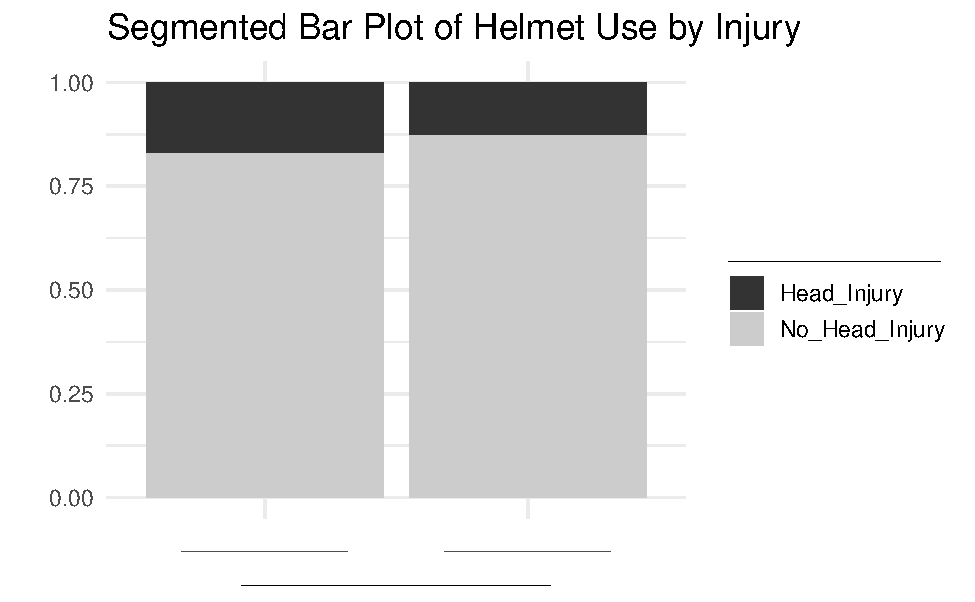
\includegraphics[width=0.7\linewidth]{07-inference-2cat_files/figure-latex/unnamed-chunk-2-1} \end{center}

\begin{enumerate}
\def\labelenumi{\arabic{enumi}.}
\setcounter{enumi}{11}
\tightlist
\item
  Fill in the blanks on the graph with the appropriate variables and values to plot a segmented bar plot of injury by helmet use.
\end{enumerate}

\vspace{1in}

\begin{enumerate}
\def\labelenumi{\arabic{enumi}.}
\setcounter{enumi}{12}
\tightlist
\item
  Based on the bar plot, Does there appear to be an association between helmet use and head injury? Explain.
\end{enumerate}

\vspace{1in}

\begin{enumerate}
\def\labelenumi{\arabic{enumi}.}
\setcounter{enumi}{13}
\tightlist
\item
  Calculate the point estimate for this study. We will use helmet use minus no helmet use as the order of subtraction.
\end{enumerate}

\vspace{1in}

\begin{enumerate}
\def\labelenumi{\arabic{enumi}.}
\setcounter{enumi}{14}
\tightlist
\item
  What is the notation used for the value calculated in question 14?
\end{enumerate}

\vspace{0.5in}

\hypertarget{use-statistical-analysis-methods-to-draw-inferences-from-the-data}{%
\section{Use statistical analysis methods to draw inferences from the data}\label{use-statistical-analysis-methods-to-draw-inferences-from-the-data}}

To test the null hypothesis we could use simulation methods as we did with a single categorical variable. In this activity we will focus on theory-based methods. Like with a single proportion, the difference in proportions can be mathematically modeled using the normal distribution if certain conditions are met.

Conditions for the sample distribution of \(\hat{p}_1-\hat{p}_2\)

\begin{itemize}
\item
  Independence: The data are independent within and between the two groups.
\item
  Success-Failure Condition: The success-failure condition holds for each group.
\end{itemize}

\vspace{.25in}

\begin{enumerate}
\def\labelenumi{\arabic{enumi}.}
\setcounter{enumi}{15}
\tightlist
\item
  Is the independence condition met? Explain your answer.
\end{enumerate}

\vspace{1in}

\begin{enumerate}
\def\labelenumi{\arabic{enumi}.}
\setcounter{enumi}{16}
\tightlist
\item
  Is the success-failure condition met for each group? Explain your answer.
\end{enumerate}

\vspace{1in}

To calculate the test statistic we use:

\begin{center}
    $Z = \frac{\text{point estimate} - \text{null value}}{SE}$

where the standard error is calculated using the pooled proportion of successes.

   $SE(\hat{p}_1-\hat{p}_2)=\sqrt{\hat{p}_{pool}(1-\hat{p}_{pool})(\frac{1}{n_1}+\frac{1}{n_2})}, \text{where}$ 
    
   $\hat{p}_{pool} = \frac{\text{number of "successes"}}{\text{number of cases}} = \frac{\hat{p}_1 n_1+\hat{p}_2 n_2}{n_1+n_2}$
    
\end{center}

\vspace{.25in}

\begin{enumerate}
\def\labelenumi{\arabic{enumi}.}
\setcounter{enumi}{17}
\tightlist
\item
  Calculate the \(SE(\hat{p}_1-\hat{p}_2)\).
\end{enumerate}

\vspace{1in}

\begin{enumerate}
\def\labelenumi{\arabic{enumi}.}
\setcounter{enumi}{18}
\tightlist
\item
  Calculate the test statistic.
\end{enumerate}

\vspace{1in}

We will use the pnorm function in R to find the p-value.

\begin{verbatim}
#> [1] 0.002118205
\end{verbatim}

\begin{enumerate}
\def\labelenumi{\arabic{enumi}.}
\setcounter{enumi}{19}
\item
  Report the p-value.
  \vspace{0.5in}
\item
  How much evidence does the p-value provide against the null hypothesis?
\end{enumerate}

\vspace{0.5in}

To find a confidence interval for the difference in proportions we will add and subtract the margin of error from the point estimate to find the two endpoints.

\[\hat{p}_1-\hat{p}_2\pm z^*SE(\hat{p}_1-\hat{p}_2), \text{where}\]

\[SE(\hat{p}_1-\hat{p}_2) = \sqrt{\left(\frac{\hat{p}_1 (1-\hat{p}_1)}{n_1}+\frac{\hat{p}_2 (1-\hat{p}_2)}{n_2}\right)}\]

Note that the formula changes when calculating the variability around the statistic in order to calculate a confidence interval! Here use the sample proportions for each group to calculate the standard error for the difference in proportions. The \(z^*\) multiplier is found under the normal distribution. We find the values that encompass the middle 95\% of the data.

\begin{verbatim}
#> [1] 1.959964
\end{verbatim}

\begin{enumerate}
\def\labelenumi{\arabic{enumi}.}
\setcounter{enumi}{21}
\tightlist
\item
  Calculate the standard error for a difference in proportions to create a 95\% confidence interval.
\end{enumerate}

\vspace{1in}

\begin{enumerate}
\def\labelenumi{\arabic{enumi}.}
\setcounter{enumi}{22}
\tightlist
\item
  Using the multiplier of \(z^*\) = 1.96, calculate the 95\% confidence interval for the difference in true proportion of head injuries for those that used helmets minus those who did not.
\end{enumerate}

\vspace{1in}

\begin{enumerate}
\def\labelenumi{\arabic{enumi}.}
\setcounter{enumi}{23}
\tightlist
\item
  Interpret the confidence interval found in question 23 in context of the problem.
\end{enumerate}

\vspace{1in}

\begin{enumerate}
\def\labelenumi{\arabic{enumi}.}
\setcounter{enumi}{24}
\tightlist
\item
  Write a paragraph summarizing the results of the study. Be sure to include:
\end{enumerate}

\begin{itemize}
\item
  Summary statistic
\item
  P-value
\item
  Conclusion (written to answer the research question)
\item
  Confidence interval
\item
  Interpretation of the confidence interval
\item
  Scope of inference
\end{itemize}

\vspace{3in}

\hypertarget{types-of-errors}{%
\section{Types of Errors}\label{types-of-errors}}

Hypothesis tests are not flawless. In a hypothesis test, there are two competing hypotheses: the null and alternative. We make a decision about which might be true, but we may choose incorrectly.

\begin{longtable}[]{@{}ccll@{}}
\toprule
& & Test Conclusion &\tabularnewline
\midrule
\endhead
Truth & \(H_0\) true & good decision & Type 1 Error\tabularnewline
& \(H_A\) true & Type 2 Error & good decision\tabularnewline
\bottomrule
\end{longtable}

A Type 1 Error is rejecting the null hypothesis when \(H_0\)is actually true. A Type 2 Error is failing to reject the null hypothesis when the alternative is actually true.

\begin{enumerate}
\def\labelenumi{\arabic{enumi}.}
\setcounter{enumi}{25}
\tightlist
\item
  Using a significance level of 0.05, what decision do you make in regards to the null hypothesis?
\end{enumerate}

\vspace{0.5in}

\begin{enumerate}
\def\labelenumi{\arabic{enumi}.}
\setcounter{enumi}{26}
\tightlist
\item
  What type of error could we have made?
\end{enumerate}

\vspace{0.5in}

\begin{enumerate}
\def\labelenumi{\arabic{enumi}.}
\setcounter{enumi}{27}
\tightlist
\item
  Write this error in context of the problem.
\end{enumerate}

\vspace{1in}

\hypertarget{statistical-investigations-for-paired-data}{%
\chapter{Statistical Investigations for Paired Data}\label{statistical-investigations-for-paired-data}}

\hypertarget{learning-outcomes}{%
\section{Learning Outcomes}\label{learning-outcomes}}

\begin{itemize}
\item
  Given a research question, construct the null and alternative hypotheses
  in words and using appropriate statistical symbols
\item
  Describe and perform simulation-based hypothesis
\item
  Interpret and evaluate a p-value
\item
  Construct and interpret a theory-based confidence interval
\item
  Use a confidence interval to determine the conclusion of a hypothesis test
\end{itemize}

\hypertarget{mean-difference-in-heart-rates-for-jumping-jacks-and-bicycle-kicks}{%
\section{Mean Difference in Heart Rates for Jumping Jacks and Bicycle Kicks}\label{mean-difference-in-heart-rates-for-jumping-jacks-and-bicycle-kicks}}

Which exercise, jumping jacks or bicycle kicks will raise your heart rate more? Students in an introductory statistics class were asked to participate in an experiment to answer this question. Each student flipped a coin to determine which exercise to complete first. If the coin landed on heads the student would do jumping jacks for 30 seconds and then measure their heart rate. After a 2 minute break the student would do bicycle kicks for 30 seconds and then record their heart rate. If the coin landed on tails the student would complete bicycle kicks first followed by jumping jacks using the same times as above.

\hypertarget{review}{%
\section{Review}\label{review}}

\begin{center}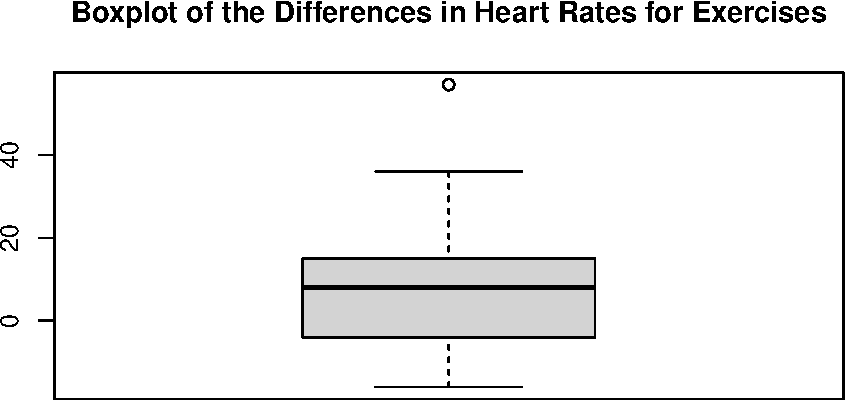
\includegraphics[width=0.7\linewidth]{08-paired_files/figure-latex/unnamed-chunk-1-1} \end{center}

\begin{verbatim}
#>  min Q1 median Q3 max     mean       sd  n missing
#>  -16 -4      8 15  57 7.604651 15.91666 43       0
\end{verbatim}

\begin{enumerate}
\def\labelenumi{\arabic{enumi}.}
\tightlist
\item
  What is the sample size?
\end{enumerate}

\vspace{0.5in}

\begin{enumerate}
\def\labelenumi{\arabic{enumi}.}
\setcounter{enumi}{1}
\tightlist
\item
  Identify the variables in this study. What role do each have?
\end{enumerate}

\vspace{1in}

\begin{enumerate}
\def\labelenumi{\arabic{enumi}.}
\setcounter{enumi}{2}
\tightlist
\item
  Why is this treated as a paired study design and not two independent samples?
\end{enumerate}

\vspace{1in}

\begin{enumerate}
\def\labelenumi{\arabic{enumi}.}
\setcounter{enumi}{3}
\tightlist
\item
  What is the purpose of randomizing the order of jumping jacks and bicycle kicks before measuring heart rates?
\end{enumerate}

\vspace{1in}

\hypertarget{ask-a-research-question}{%
\section{Ask a Research Question}\label{ask-a-research-question}}

\begin{enumerate}
\def\labelenumi{\arabic{enumi}.}
\setcounter{enumi}{4}
\tightlist
\item
  What are the two competing possibilities to run a hypothesis test?
\end{enumerate}

\vspace{1in}

\begin{enumerate}
\def\labelenumi{\arabic{enumi}.}
\setcounter{enumi}{5}
\tightlist
\item
  Write the null hypothesis in words.
\end{enumerate}

\vspace{1in}

\begin{enumerate}
\def\labelenumi{\arabic{enumi}.}
\setcounter{enumi}{6}
\tightlist
\item
  What is the research question?
\end{enumerate}

\vspace{1in}

\begin{enumerate}
\def\labelenumi{\arabic{enumi}.}
\setcounter{enumi}{7}
\tightlist
\item
  Write the alternative hypothesis in notation.
\end{enumerate}

\vspace{1in}

\hypertarget{summarize-and-visualize-the-data}{%
\section{Summarize and Visualize the Data}\label{summarize-and-visualize-the-data}}

\begin{enumerate}
\def\labelenumi{\arabic{enumi}.}
\setcounter{enumi}{8}
\tightlist
\item
  Report the summary statistic for the data.
\end{enumerate}

\vspace{0.5in}

\begin{enumerate}
\def\labelenumi{\arabic{enumi}.}
\setcounter{enumi}{9}
\tightlist
\item
  What notation is used for the value in question 9?
\end{enumerate}

\vspace{0.5in}

\hypertarget{use-statistical-inferential-methods-to-draw-inferences-from-the-data}{%
\section{Use statistical inferential methods to draw inferences from the data}\label{use-statistical-inferential-methods-to-draw-inferences-from-the-data}}

To simulate the null distribution we will use a bootstrapping method - sampling with replacement from the data set. Before bootstrapping we will need to shift the each data point by the difference \(\mu_0 - \bar{x}\). This will ensure that the simulated null distribution will be centered at the null value.

\begin{enumerate}
\def\labelenumi{\arabic{enumi}.}
\setcounter{enumi}{10}
\tightlist
\item
  Calculate the difference \(\mu_0 - \bar{x}\). Will we need to shift the data up or down?
\end{enumerate}

\vspace{1in}

\textbf{Add simulation here}

\begin{enumerate}
\def\labelenumi{\arabic{enumi}.}
\setcounter{enumi}{11}
\tightlist
\item
  Explain why the null distribution is centered at zero.
\end{enumerate}

\vspace{1in}

\begin{enumerate}
\def\labelenumi{\arabic{enumi}.}
\setcounter{enumi}{12}
\tightlist
\item
  What proportion of samples are beyond the sample mean difference in heart beats for jumping jacks minus bicycle kicks?
\end{enumerate}

\vspace{1in}

\hypertarget{communicate-the-results-and-answer-the-research-question.}{%
\section{Communicate the results and answer the research question.}\label{communicate-the-results-and-answer-the-research-question.}}

\begin{enumerate}
\def\labelenumi{\arabic{enumi}.}
\setcounter{enumi}{13}
\tightlist
\item
  Write out the parameter of interest in context of the study.
\end{enumerate}

\vspace{1in}

To calculate a confidence interval to estimate the mean difference in heart rates, we will use this equation:

\(\bar{x}_d \pm t^*SE(\bar{x}_d)\), where \(SE(\bar{x}_d) = \sqrt(\frac{\bar{x}_d}{n_d})\)

To find the \(t^*\) multiplier for a 95\% confidence interval we will find the value in the t-distribution that represents the endpoints for the middle 95\% of the data.

\begin{verbatim}
#> [1] 2.018082
\end{verbatim}

\begin{enumerate}
\def\labelenumi{\arabic{enumi}.}
\setcounter{enumi}{14}
\tightlist
\item
  Calculate the \(SE(\bar{x}_d)\).
\end{enumerate}

\vspace{1in}

\begin{enumerate}
\def\labelenumi{\arabic{enumi}.}
\setcounter{enumi}{15}
\tightlist
\item
  Calculate a 95\% confidence interval for the parameter of interest.
\end{enumerate}

\vspace{1in}

\begin{enumerate}
\def\labelenumi{\arabic{enumi}.}
\setcounter{enumi}{16}
\tightlist
\item
  Interpret the 95\% confidence interval in context of the problem.
\end{enumerate}

\vspace{1in}

\begin{enumerate}
\def\labelenumi{\arabic{enumi}.}
\setcounter{enumi}{17}
\tightlist
\item
  Based off your p-value and confidence interval, write a conclusion.
\end{enumerate}

\vspace{1in}

\hypertarget{revisit-and-look-forward}{%
\section{Revisit and Look Forward}\label{revisit-and-look-forward}}

Suppose we had a sample of 90 students instead of 43 resulting in the same summary statistic.

\begin{enumerate}
\def\labelenumi{\arabic{enumi}.}
\setcounter{enumi}{18}
\tightlist
\item
  Would this new data provide more or less evidence against the null hypothesis? Explain your answer.
\end{enumerate}

\vspace{1in}

\begin{enumerate}
\def\labelenumi{\arabic{enumi}.}
\setcounter{enumi}{19}
\tightlist
\item
  Would this result in a wider or narrower confidence interval?
\end{enumerate}

\vspace{1in}

\end{document}
